%!TEX root = ../dissertation.tex

\chapter{Tests and Results} \label{cha:test}

\section{Assembling Objects Test}\label{sec:ass_objs_test}

The torque reaction arm is ergonomic solution, basically a mechanical device, developed to absorb the reaction torque generated by the associated industrial tools, such as electronic and electric screwdrivers.
Torque reaction arms protect the operator from vibrations and reaction torques, improving safety in the workplace and preventing musculoskeletal disorders. \\
There are different types of arms, the assembly proposed here will compose a part of an BNP orthogonal torque reaction arms (BRF series, Figure \ref{fig:brf}). \\
Orthogonal torque reaction arms can be installed on the workbench thanks to the vertical sliding column that allows the arm to rotate around its axis. 
This arm allow orthogonal tightening operations to be performed to workbench plane. \\

The Table \ref{tab:ass_table} summarises the characteristics of the components that will be used: the Number, which is used in the figures below to indicate the component, the Quantity, the Colour Cube, which associates each component with a colour of the cube representing it (to better understand the simulation figures) and the Semantic Name, which is the name given to each component and which is used in the AtomSpace.

\begin{table}[H]
  \centering
  \caption{Assemblable Objects Description Table}\label{tab:ass_table}
  \medskip
\renewcommand\arraystretch{1.5}
\renewcommand\tabcolsep{12pt}
\begin{tabular}{cccc}
\toprule
\multicolumn{4}{c}{\textbf{Assemblable Objects}} \\
\textbf{Number} &  \textbf{Quantity} &  \textbf{Colour Cube} &  \textbf{Semantic Name}  \\
\midrule
\rowcolor{gray!25}
5 & 2 & Green / Orange & BearingSleeve1 / BearingSleeve2 \\
6 & 1 & Blue & BettClamp \\
\rowcolor{gray!25}
7 & 1 & - & Bearing \\
9 & 2 & Grey / Gold & SnapRing1 / SnapRing2 \\
\rowcolor{gray!25}
14 & 1 & - & TCEIScrew \\
31 & 1 & - & RotatingBalancerSupport \\
\rowcolor{gray!25}
32 & 1 & Red & RecirculatingBallSleeve \\
39 & 1 & - & UpperBearingBracket \\
\rowcolor{gray!25}
43 & 1 & Yellow & InductionHardenedRod \\
\bottomrule
\end{tabular}
\end{table}

\begin{figure} [h]
\centering
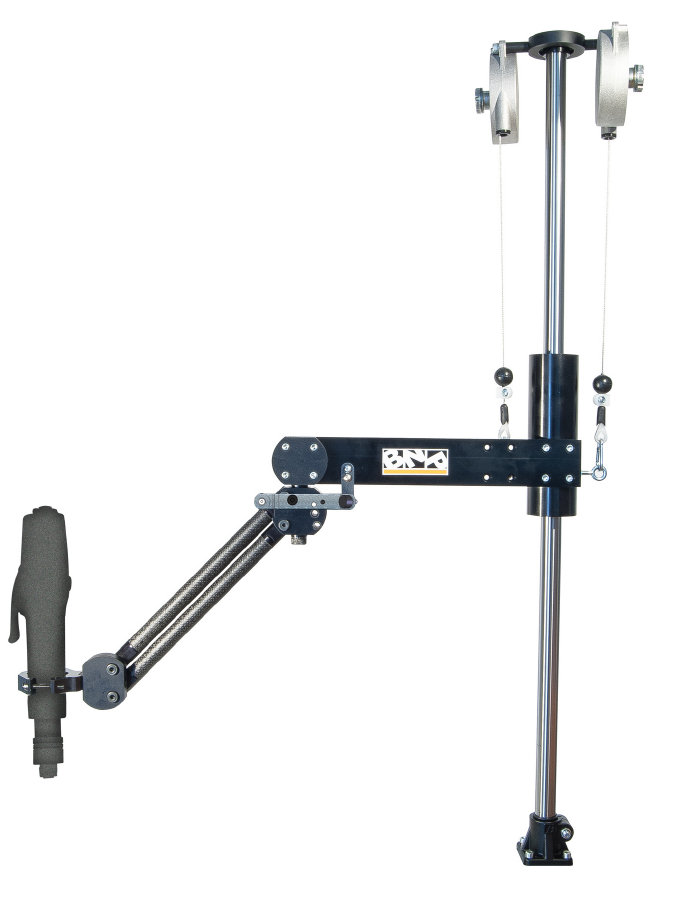
\includegraphics[width=0.5
\textwidth]{figures/Magistrale/BRF}
\caption[BNP Orthogonal Torque Reaction Arms]{BNP orthogonal torque reaction arms, BRF series. Folded arm which allows orthogonal tightening to workbench plane.
\label{fig:brf}}
\end{figure} 

The arm assembly is schematically shown in Figure \ref{fig:brf_draw} and has been divided into three sub-assemblies:

\begin{enumerate}
	\item BlockA: the Bett clamp and the induction hardened rod are taken from their respective bins and mounted on top of the workbench (Figure \ref{fig:ass_obj_1}). Next, the resulting component will be called BlockA and will be represented by a single cube. Finally, it will be moved from the workbench to the table

	\item BlockB: Once the workbench is freed, the second piece is assembled, using two snap rings, two bearing sleeves and one recirculating ball sleeve (Figure \ref{fig:ass_obj_2}). It will be called BlockB and will then be assembled with BlockA (\enquote{stack BlockA BlockB}) above the table

	\item BlockC: Finally, the last component, consisting of an upper bearing bracket, a bearing, a rotating balancer support and a TCEI screw, is mounted (Figure \ref{fig:ass_obj_2}). This will be BlockC and will be stacked on top of BlockB
\end{enumerate}

The block assembly tables describe the steps that are performed to create BlocksA, BlocksB and BlocksC. A description of their parameters is as follows:

\begin{itemize}
	\item Objects List: this is the list of objects that have been detected through the AprilTags or extracted from the additional information
	\item Additional Info.: each line corresponds to a sentence inserted during the learning phase
	\item Request: each line corresponds to a sentence inserted during the request phase, that is a goal to be reached
	\item Solution: each line corresponds to an action that is executed. These scripts are both the exact lines of Scheme code used to call the respective rules in Atomese, and the information passed to the ROS client, after the search phase, to move the robot
	\item Exec. Time: execution time of the search phase. It does not include any of the other phases and indeed corresponds to the time needed to expand the tree until a solution is found.
	\item No. Iters: number of recursive calls performed by the algorithm
\end{itemize} 

It is important to point out a few considerations concerning this test. First of all, the concept of \enquote{assembly} in this project simply corresponds to a stack action. \\
Assembly took place in a simulated environment, starting with the configuration shown in Figure \ref{fig:ass_1}. 
Inside each bin, there are one or more cubes representing assemblable objects. Objects without Colour Cube (i.e. those in BlockC) are not shown in the simulation figures, both because BlockC is assembled in a similar way to BlockB, and to keep the illustrations clearer. \\
Moreover, BlockA is solved in two runs of the algorithm (Tables \ref{tab:ass_A_1} and \ref{tab:ass_A_2}). 
The first one assembles the objects and the second one reconsiders them as a single cube and moves it. This is because the environment and \enquote{senses} of the robot are simplified, thus, the cubes do not \enquote{join} together and it is not possible to pick up two or more at a time. \\
For example, BlockA, which is mounted on the workbench and then moved to the table, could be mounted directly on the table. However, a future development of the system may be able to work with real objects, which means real assemblies (and not just stacking), grabbing complex objects, etc.. Therefore, the first way was preferred and is also valid for BlockB and BlockC (Tables \ref{tab:ass_B_4} and \ref{tab:ass_C_3}). \\
Another consideration concerns multiple executions of the algorithm to solve BlockB and BlockC. It has not been possible to solve these two assemblies with one request phase each, due to hardware performance (see Section \ref{sec:perf_consid}). Consequently, the problems were split into smaller requests and solved sequentially. The final arrangement is still achieved, but multiple runs of the algorithm also imply multiple execution times of each of its phases.
Excluding the last run to move the single cube, BlockB required three runs of the algorithm (Tables \ref{tab:ass_B_1}, \ref{tab:ass_B_2}, \ref{tab:ass_B_3}), while BlockC required two (Tables \ref{tab:ass_C_1}, \ref{tab:ass_C_2}). \\
The last figures represent the execution of the test in the simulated environment for BlockA and BlockB:
\begin{enumerate}
	\item The test starts with Figure \ref{fig:ass_1}
	\item In Figure \ref{fig:ass_2}, the components of BlockA are assembled on top of the workbench 
	\item Their respective cubes are manually replaced with a single cube (the yellow one), and finally it is moved over the table
	\item Next, the first two components of BlockB are stacked (first split, Table \ref{tab:ass_B_1}) as in Figure \ref{fig:ass_3}
	\item Finally in Figure \ref{fig:ass_4}, the second two components (second split, Table \ref{tab:ass_B_2}) and then the last one (third split, Table \ref{tab:ass_B_3}) are assembled. 
	\item The final step, where the cubes are manually replaced with a single one that will be stacked on blockA, is omitted
\end{enumerate}
	
\begin{table}[htbp]
  \centering
  \caption{BlockA Assembly Process}\label{tab:ass_A_1}
  \medskip
\renewcommand\arraystretch{1}
\renewcommand\tabcolsep{5pt}
\begin{tabular}{ll}
\toprule
\textbf{Parameters} &  \textbf{Values}  \\
\midrule
\rowcolor{gray!25}
Objects List &  InductionHardenedRod, BettClamp, SnapRing1, \\
\rowcolor{gray!25}
& RecirculatingBallSleeve, BearingSleeve1, BearingSleeve2, table, \\
\rowcolor{gray!25}
& workbench, PurpleBin, GreenBin, RedBin, BlueBin, YellowBin \\
Additional Info. & The table is a fixed object. \\
& The workbench is a fixed object. \\
& The PurpleBin is a fixed object. \\
& The GreenBin is a fixed object. \\
& The RedBin is a fixed object. \\
& The BlueBin is a fixed object. \\
& The YellowBin is a fixed object. \\
& The SnapRing1 is on the SnapRing2. \\
& The BearingSleeve1 is on the BearingSleeve2. \\
\rowcolor{gray!25}
Request & The BettClamp is on the workbench. \\
\rowcolor{gray!25}
& The InductionHardenedRod is on the BettClamp. \\
Solution & (pickup (ConceptNode "BettClamp")) \\
& (stack (ConceptNode "BettClamp") (ConceptNode "workbench")) \\
& (pickup (ConceptNode "InductionHardenedRod")) \\
& (stack (ConceptNode "InductionHardenedRod") (ConceptNode "BettClamp")) \\
\rowcolor{gray!25}
Exec. Time & 25 sec \\
No. Iters. & 401 \\	
\bottomrule
\end{tabular}
\end{table}

\begin{table}[htbp]
  \centering
  \caption{BlockA Move Process}\label{tab:ass_A_2}
  \medskip
\begin{tabular}{ll}
\toprule
\textbf{Parameters} &  \textbf{Values}  \\
\midrule
\rowcolor{gray!25}
Objects List &  BlockA, SnapRing1, SnapRing2, RecirculatingBallSleeve, \\
\rowcolor{gray!25}
& BearingSleeve1, BearingSleeve2, table, workbench, \\
\rowcolor{gray!25}
&  PurpleBin, GreenBin, RedBin, BlueBin, YellowBin \\
Additional Info. & \footnotemark{} \\
& The SnapRing1 is on the SnapRing2. \\
& The BearingSleeve1 is on the BearingSleeve2. \\
\rowcolor{gray!25}
Request & The BlockA is on the table. \\
Solution & (pickup (ConceptNode "BlockA")) \\
& (stack (ConceptNode "BlockA") (ConceptNode "table")) \\
\rowcolor{gray!25}
Exec. Time & 0 sec \\
No. Iters. & 3 \\	
\bottomrule
\end{tabular}
\end{table}

\begin{table}[htbp]
  \centering
  \caption{BlockB Assembly Process 1}\label{tab:ass_B_1}
  \medskip
\begin{tabular}{ll}
\toprule
\textbf{Parameters} &  \textbf{Values}  \\
\midrule
\rowcolor{gray!25}
Objects List &  BlockA, SnapRing1, SnapRing2, RecirculatingBallSleeve, \\
\rowcolor{gray!25}
& BearingSleeve1, BearingSleeve2, table, workbench, \\
\rowcolor{gray!25}
&  PurpleBin, GreenBin, RedBin, BlueBin, YellowBin \\
Additional Info. & \footnotemark{} \\
& The SnapRing1 is on the SnapRing2. \\
& The BearingSleeve1 is on the BearingSleeve2. \\
\rowcolor{gray!25}
Request & The SnapRing1 is on the workbench. \\
\rowcolor{gray!25}
& The BearingSleeve1 is on the SnapRing1. \\
Solution & (unstack (ConceptNode "SnapRing1") (ConceptNode "SnapRing2")) \\
& (stack (ConceptNode "SnapRing1") (ConceptNode "workbench")) \\
& (unstack (ConceptNode "BearingSleeve1")(ConceptNode "BearingSleeve2")) \\
& (stack (ConceptNode "BearingSleeve1") (ConceptNode "SnapRing1")) \\
\rowcolor{gray!25}
Exec. Time & 39 sec \\
No. Iters. & 493 \\	
\bottomrule
\end{tabular}
\end{table}

\begin{table}[htbp]
  \centering
  \caption{BlockB Assembly Process 2}\label{tab:ass_B_2}
  \medskip
\begin{tabular}{ll}
\toprule
\textbf{Parameters} &  \textbf{Values}  \\
\midrule
\rowcolor{gray!25}
Objects List &  BlockA, SnapRing1, SnapRing2, RecirculatingBallSleeve, \\
\rowcolor{gray!25}
& BearingSleeve1, BearingSleeve2, table, workbench, \\
\rowcolor{gray!25}
&  PurpleBin, GreenBin, RedBin, BlueBin, YellowBin \\
Additional Info. & \footnotemark{} \\
& The SnapRing1 is on the workbench. \\
& The BearingSleeve1 is on the SnapRing1. \\
\rowcolor{gray!25}
Request & The RecirculatingBallSleeve is on the BearingSleeve1. \\
& The BearingSleeve2 is on the RecirculatingBallSleeve. \\
Solution & (pickup (ConceptNode "RecirculatingBallSleeve")) \\
& (stack (ConceptNode "RecirculatingBallSleeve") \\
& \quad\quad\quad(ConceptNode "BearingSleeve1")) \\
& (pickup (ConceptNode "BearingSleeve2")) \\
& (stack (ConceptNode "BearingSleeve2") \\
& \quad\quad\quad(ConceptNode "RecirculatingBallSleeve")) \\
\rowcolor{gray!25}
Exec. Time & 21 sec \\
No. Iters. & 343 \\	
\bottomrule
\end{tabular}
\end{table}

\begin{table}[htbp]
  \centering
  \caption{BlockB Assembly Process 3}\label{tab:ass_B_3}
  \medskip
\begin{tabular}{ll}
\toprule
\textbf{Parameters} &  \textbf{Values}  \\
\midrule
\rowcolor{gray!25}
Objects List &  BlockA, SnapRing1, SnapRing2, RecirculatingBallSleeve, \\
\rowcolor{gray!25}
& BearingSleeve1, BearingSleeve2, table, workbench, \\
\rowcolor{gray!25}
&  PurpleBin, GreenBin, RedBin, BlueBin, YellowBin \\
Additional Info. & \footnotemark{} \\
& The SnapRing1 is on the workbench. \\
& The BearingSleeve1 is on the SnapRing1. \\
& The RecirculatingBallSleeve is on the BearingSleeve1. \\
& The BearingSleeve2 is on the RecirculatingBallSleeve. \\
\rowcolor{gray!25}
Request & The SnapRing2 is on the BearingSleeve2. \\
Solution & (pickup (ConceptNode "SnapRing2")) \\
& (stack (ConceptNode "SnapRing2") (ConceptNode "BearingSleeve2")) \\
\rowcolor{gray!25}
Exec. Time & 0 sec \\
No. Iters. & 3 \\	
\bottomrule
\end{tabular}
\end{table}

\begin{table}[htbp]
  \centering
  \caption{BlockB Move Process}\label{tab:ass_B_4}
  \medskip
\begin{tabular}{ll}
\toprule
\textbf{Parameters} &  \textbf{Values}  \\
\midrule
\rowcolor{gray!25}
Objects List &  BlockA, BlockB, table, workbench, \\
\rowcolor{gray!25}
&  PurpleBin, GreenBin, RedBin, BlueBin, YellowBin \\
Additional Info. & \footnotemark{} \\
\rowcolor{gray!25}
Request & The BlockB is on the BlockA. \\
Solution & (pickup (ConceptNode "BlockB")) \\
& (stack (ConceptNode "BlockB") (ConceptNode "BlockA")) \\
\rowcolor{gray!25}
Exec. Time & 0 sec \\
No. Iters. & 2 \\	
\bottomrule
\end{tabular}
\end{table}

\begin{table}[htbp]
  \centering
  \caption{BlockC Assembly Process 1}\label{tab:ass_C_1}
  \medskip
\begin{tabular}{ll}
\toprule
\textbf{Parameters} &  \textbf{Values}  \\
\midrule
\rowcolor{gray!25}
Objects List &  BlockA, BlockB, TCEIScrew, UpperBearingBracket, \\
\rowcolor{gray!25}
& RotatingBalancerSupport, Bearing, table, workbench, \\
\rowcolor{gray!25}
&  PurpleBin, GreenBin, RedBin, BlueBin, YellowBin \\
Additional Info. & \footnotemark{} \\
& The BlockB is on the BlockA. \\
\rowcolor{gray!25}
Request & The UpperBearingBracket is on the BlockC. \\
\rowcolor{gray!25}
& The Bearing is on the UpperBearingBracket. \\
\rowcolor{gray!25}
& The RotatingBalancerSupport is on the Bearing. \\
Solution & (pickup (ConceptNode "UpperBearingBracket")) \\
& (stack (ConceptNode "UpperBearingBracket") (ConceptNode "BlockC")) \\
& (pickup (ConceptNode "Bearing")) \\
& (stack (ConceptNode "Bearing") (ConceptNode "UpperBearingBracket")) \\
& (pickup (ConceptNode "RotatingBalancerSupport")) \\
& (stack (ConceptNode "RotatingBalancerSupport") (ConceptNode "Bearing")) \\
\rowcolor{gray!25}
Exec. Time & 699 sec \\
No. Iters. & 5853 \\	
\bottomrule
\end{tabular}
\end{table}

\begin{table}[htbp]
  \centering
  \caption{BlockC Assembly Process 2}\label{tab:ass_C_2}
  \medskip
\begin{tabular}{ll}
\toprule
\textbf{Parameters} &  \textbf{Values}  \\
\midrule
\rowcolor{gray!25}
Objects List &  BlockA, BlockB, TCEIScrew, UpperBearingBracket, \\
\rowcolor{gray!25}
& RotatingBalancerSupport, Bearing, table, workbench, \\
\rowcolor{gray!25}
&  PurpleBin, GreenBin, RedBin, BlueBin, YellowBin \\
Additional Info. & \footnotemark{} \\
& The BlockB is on the BlockA. \\
& The UpperBearingBracket is on the BlockC. \\
& The Bearing is on the UpperBearingBracket. \\
& The RotatingBalancerSupport is on the Bearing. \\
\rowcolor{gray!25}
Request & The TCEIScrew is on the RotatingBalancerSupport. \\
Solution & (pickup (ConceptNode "TCEIScrew")) \\
& (stack (ConceptNode "TCEIScrew") \\
& \quad\quad\quad(ConceptNode "RotatingBalancerSupport")) \\
\rowcolor{gray!25}
Exec. Time & 0 sec \\
No. Iters. & 2 \\	
\bottomrule
\end{tabular}
\end{table}

\begin{table}[htbp]
  \centering
  \caption{BlockC Move Process}\label{tab:ass_C_3}
  \medskip
\begin{tabular}{ll}
\toprule
\textbf{Parameters} &  \textbf{Values}  \\
\midrule
\rowcolor{gray!25}
Objects List &  BlockA, BlockB, BlockC, table, workbench, \\
\rowcolor{gray!25}
&  PurpleBin, GreenBin, RedBin, BlueBin, YellowBin \\
Additional Info. & \footnotemark{} \\
& The BlockB is on the BlockA. \\
\rowcolor{gray!25}
Request & The BlockC is on the BlockB. \\
Solution & (pickup (ConceptNode "BlockC")) \\
& (stack (ConceptNode "BlockC") (ConceptNode "BlockB")) \\
\rowcolor{gray!25}
Exec. Time & 0 sec \\
No. Iters. & 3 \\	
\bottomrule
\end{tabular}
\end{table}

\footnotetext{table, workbench, PurpleBin, GreenBin, RedBin, BlueBin, YellowBin}

\begin{figure} [h]
\centering
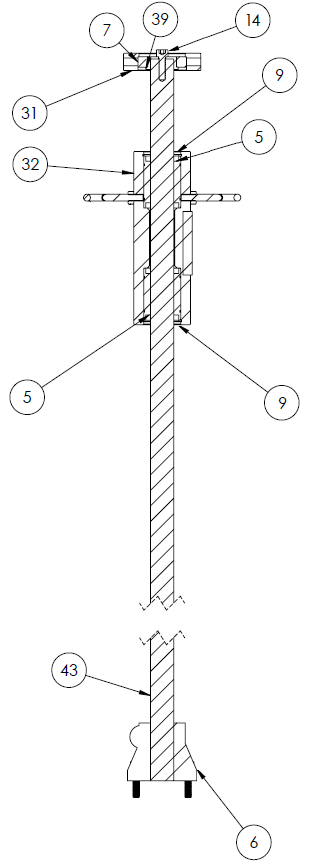
\includegraphics[width=0.25
\textwidth]{figures/Magistrale/BRF_draw}
\caption[Final Assembly Sketch]{Drawing of the complete assembly that has been carried out, corresponding to a part of the BNP orthogonal torque reaction arms.
\label{fig:brf_draw}}
\end{figure} 

\begin{figure} [h]
\centering
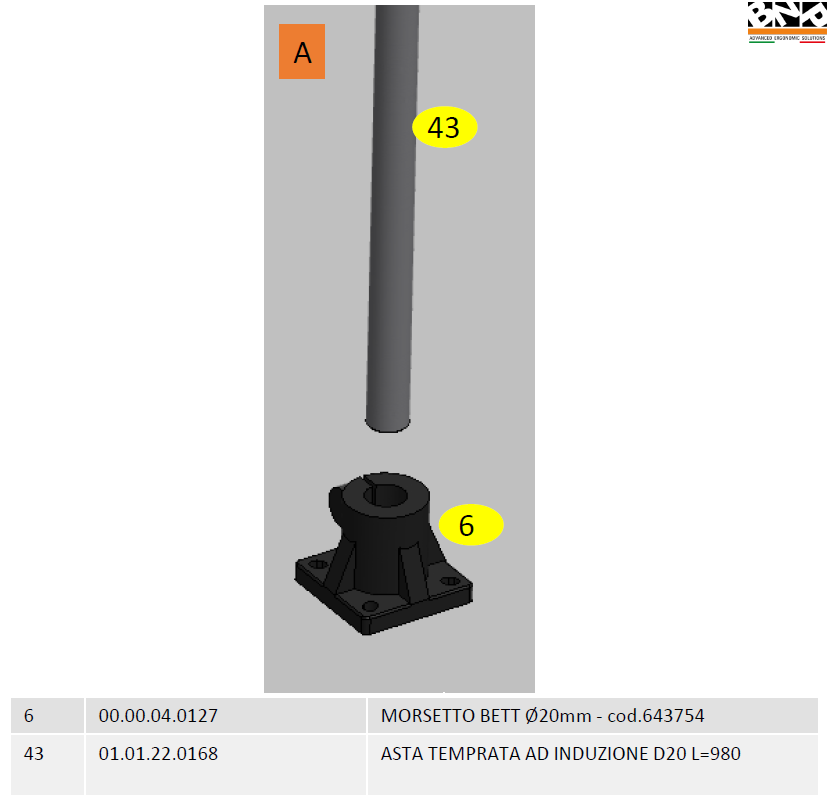
\includegraphics[width=0.6
\textwidth]{figures/Magistrale/ass_obj_1}
\caption[BlockA Assembly]{Assembly layout of BlockA
\label{fig:ass_obj_1}}
\end{figure} 

\begin{figure} [h]
\centering
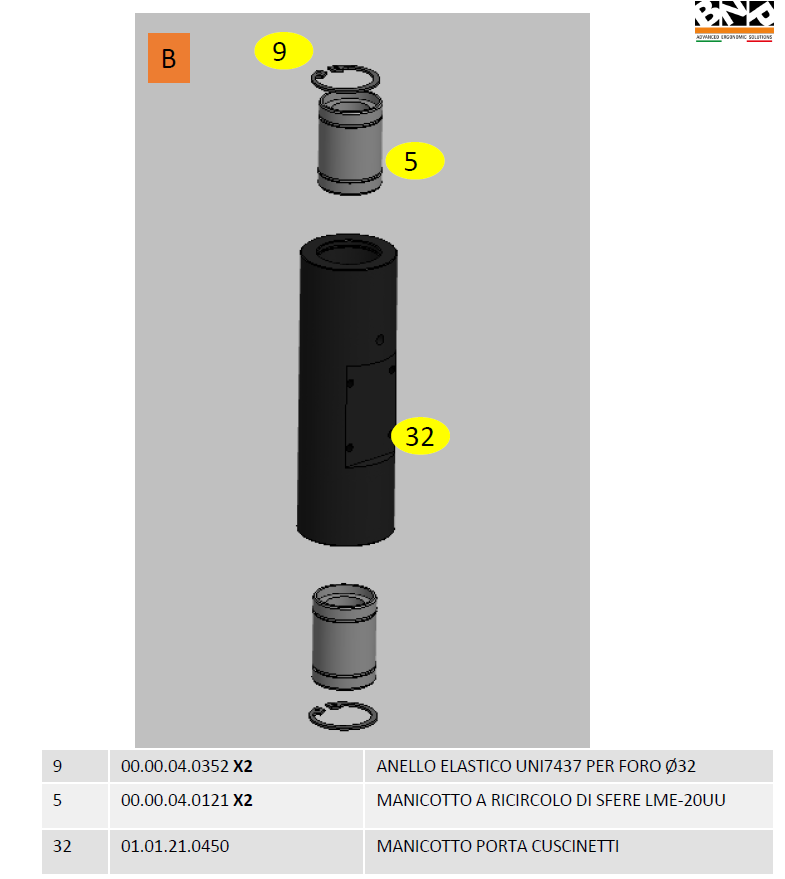
\includegraphics[width=0.6
\textwidth]{figures/Magistrale/ass_obj_2}
\caption[BlockB Assembly]{Assembly layout of BlockB
\label{fig:ass_obj_2}}
\end{figure} 

\begin{figure} [h]
\centering
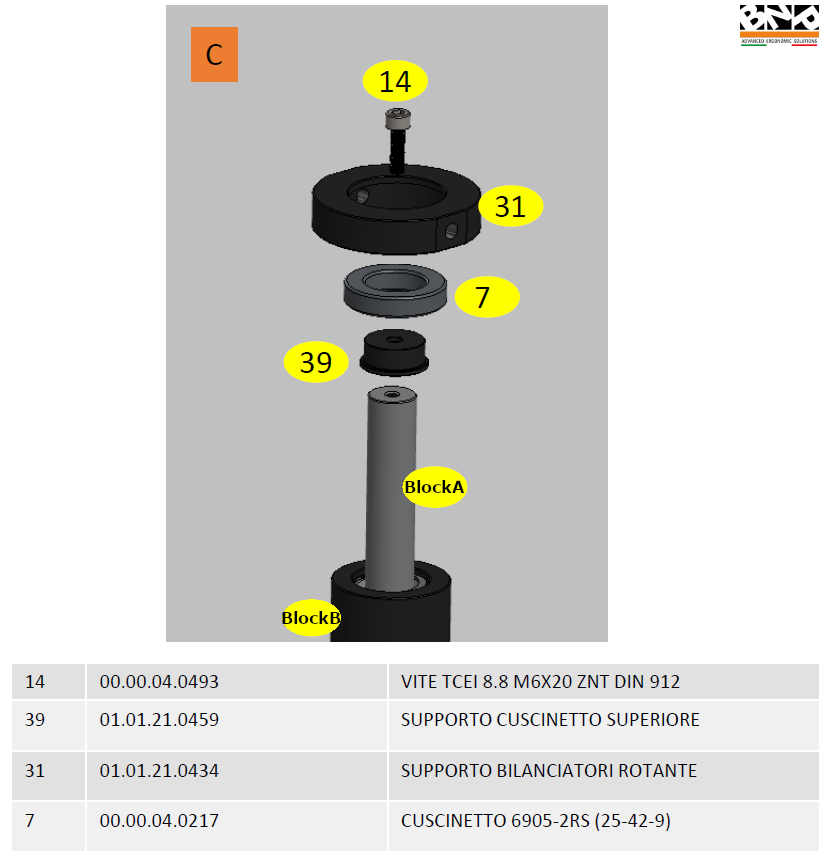
\includegraphics[width=0.6
\textwidth]{figures/Magistrale/ass_obj_3}
\caption[BlockC Assembly]{Assembly layout of BlockC
\label{fig:ass_obj_3}}
\end{figure} 

\begin{figure} [h]
\centering
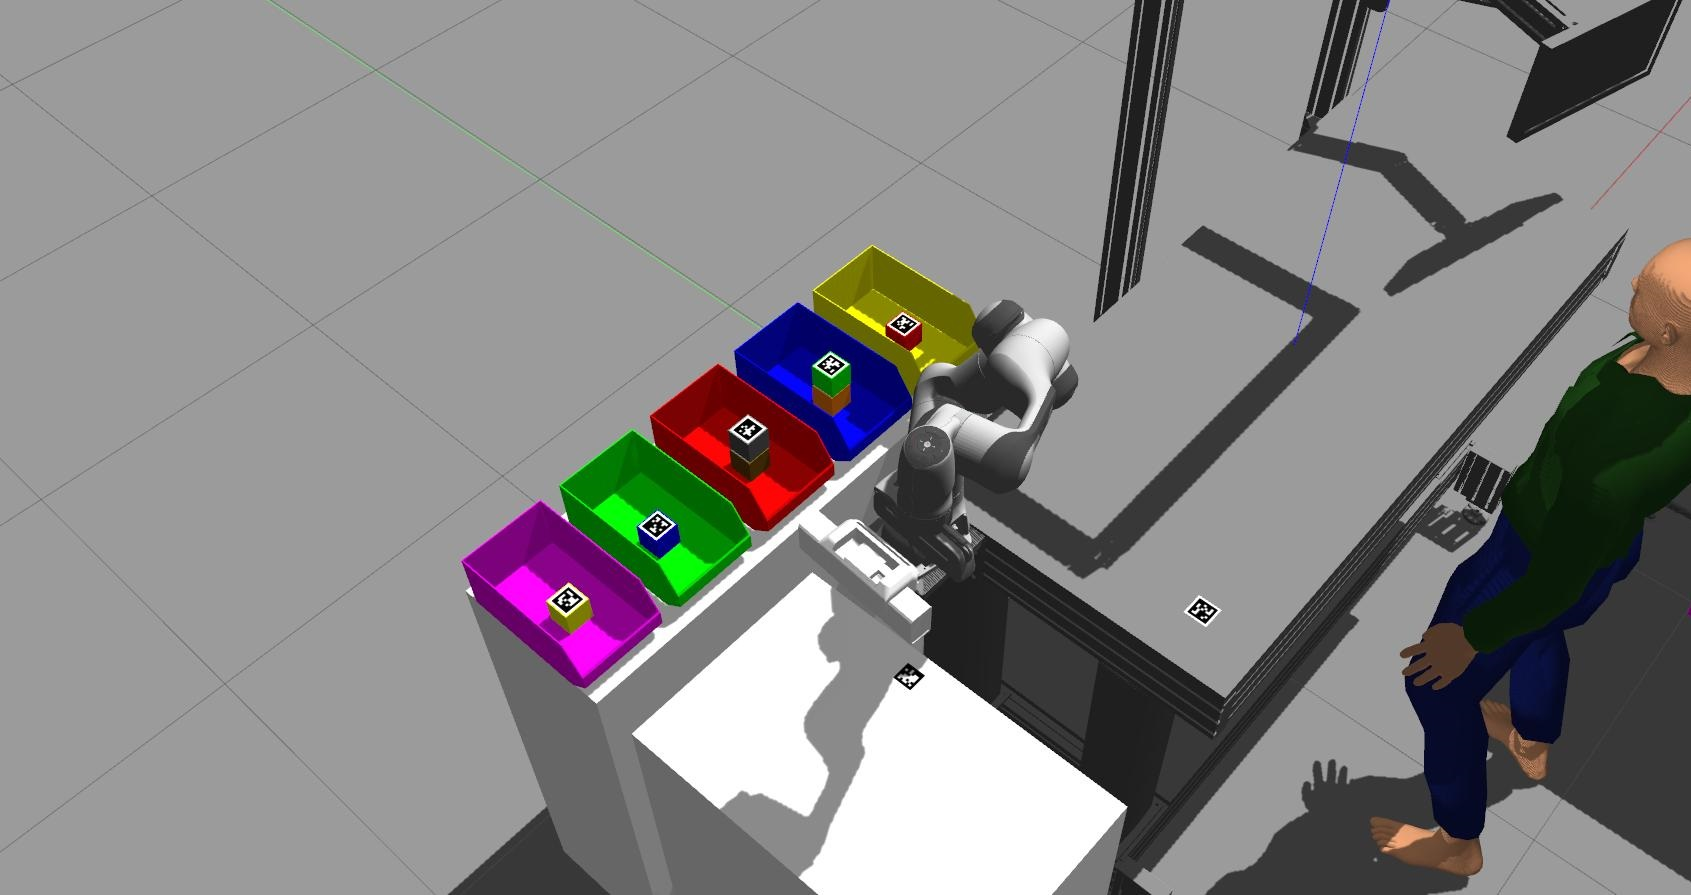
\includegraphics[width=0.6
\textwidth]{figures/Magistrale/ass_1}
\caption[Initial Assembly Test Environment]{Initial arrangement of objects in the various bins, before the robot begins the perception phase.
\label{fig:ass_1}}
\end{figure} 

\begin{figure} [h]
\centering
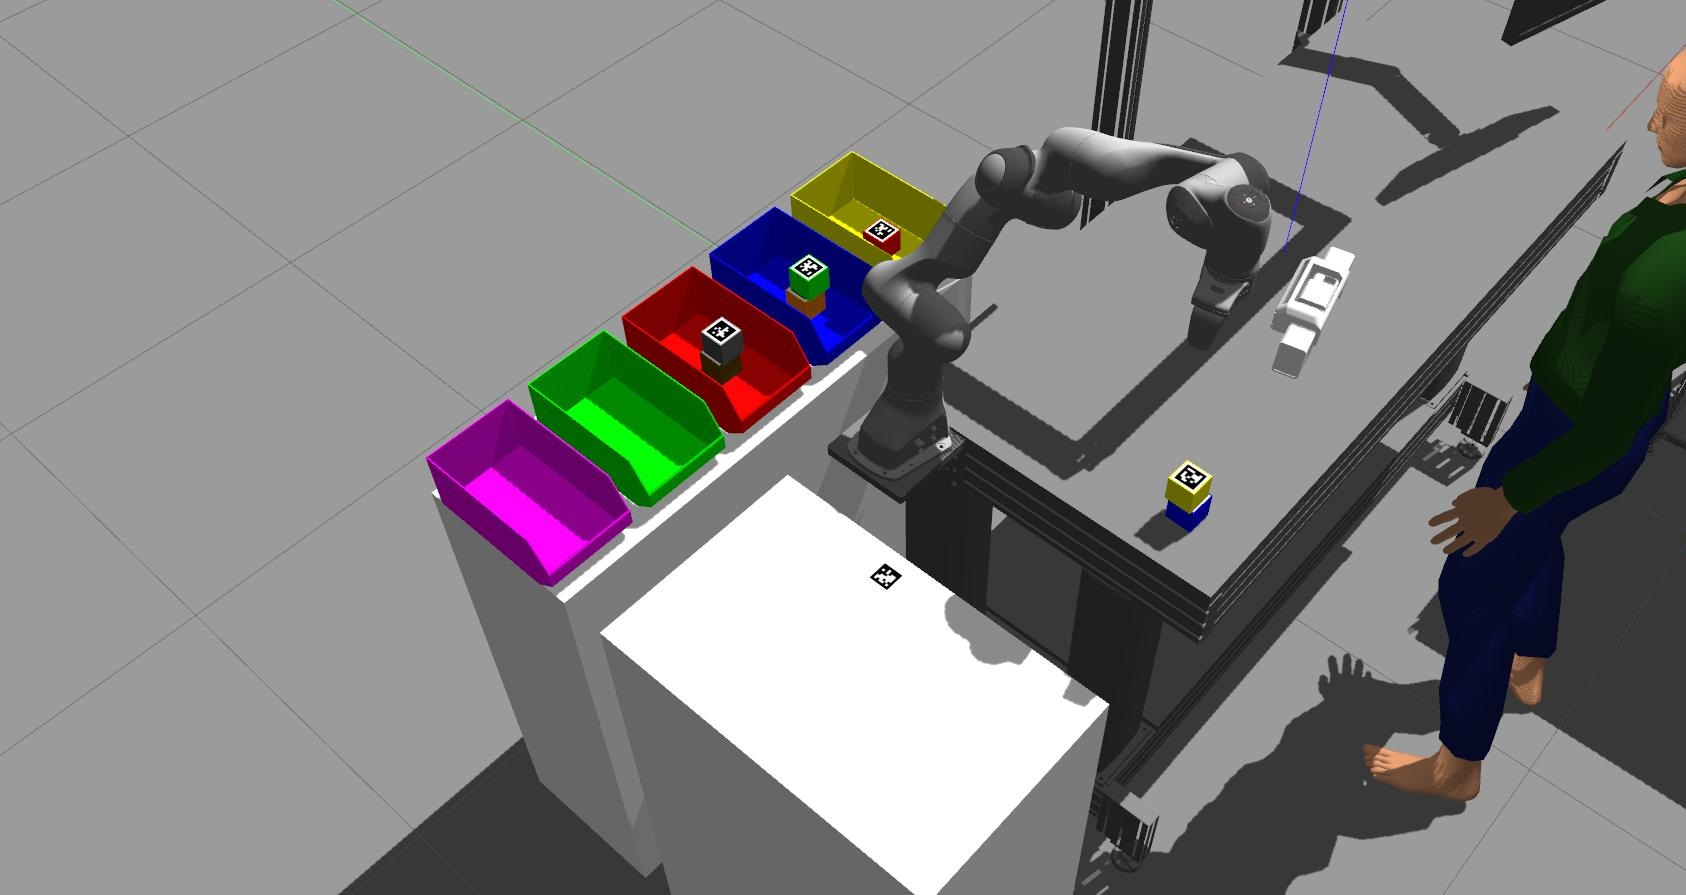
\includegraphics[width=0.6
\textwidth]{figures/Magistrale/ass_2}
\caption[BlockA Assembly Simulation]{Assembly of BlockA on the workbench completed. 
\label{fig:ass_2}}
\end{figure} 

\begin{figure} [h]
\centering
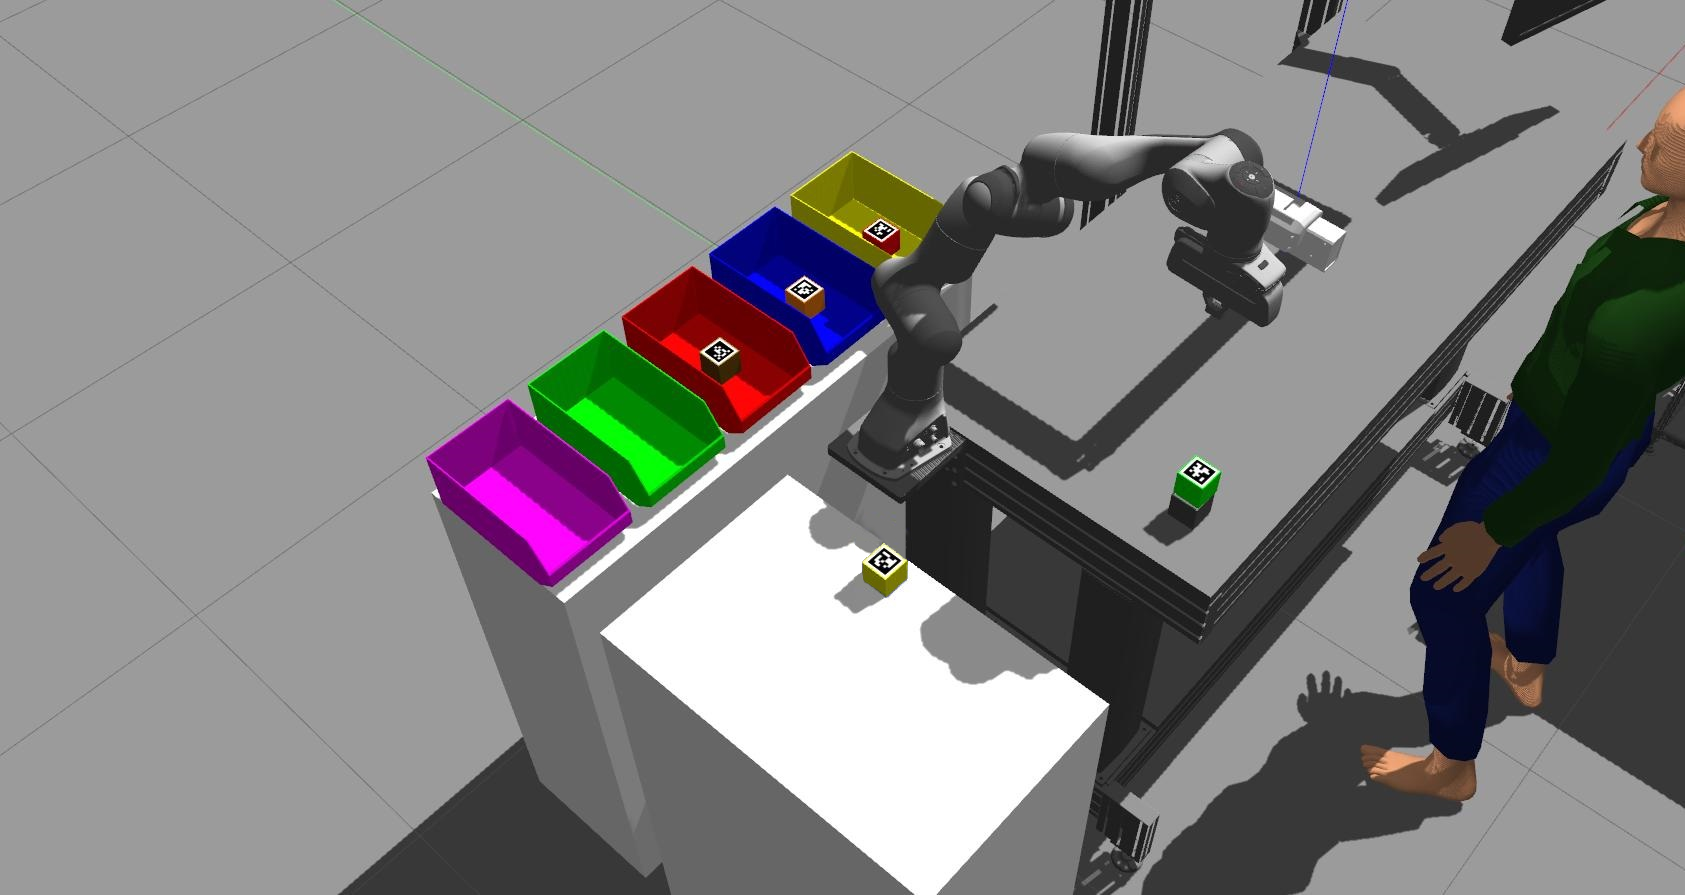
\includegraphics[width=0.6
\textwidth]{figures/Magistrale/ass_3}
\caption[First Part of BlockB Assembly Simulation]{BlockA moved over the table and first part of BlockB completed
\label{fig:ass_3}}
\end{figure} 

\begin{figure} [h]
\centering
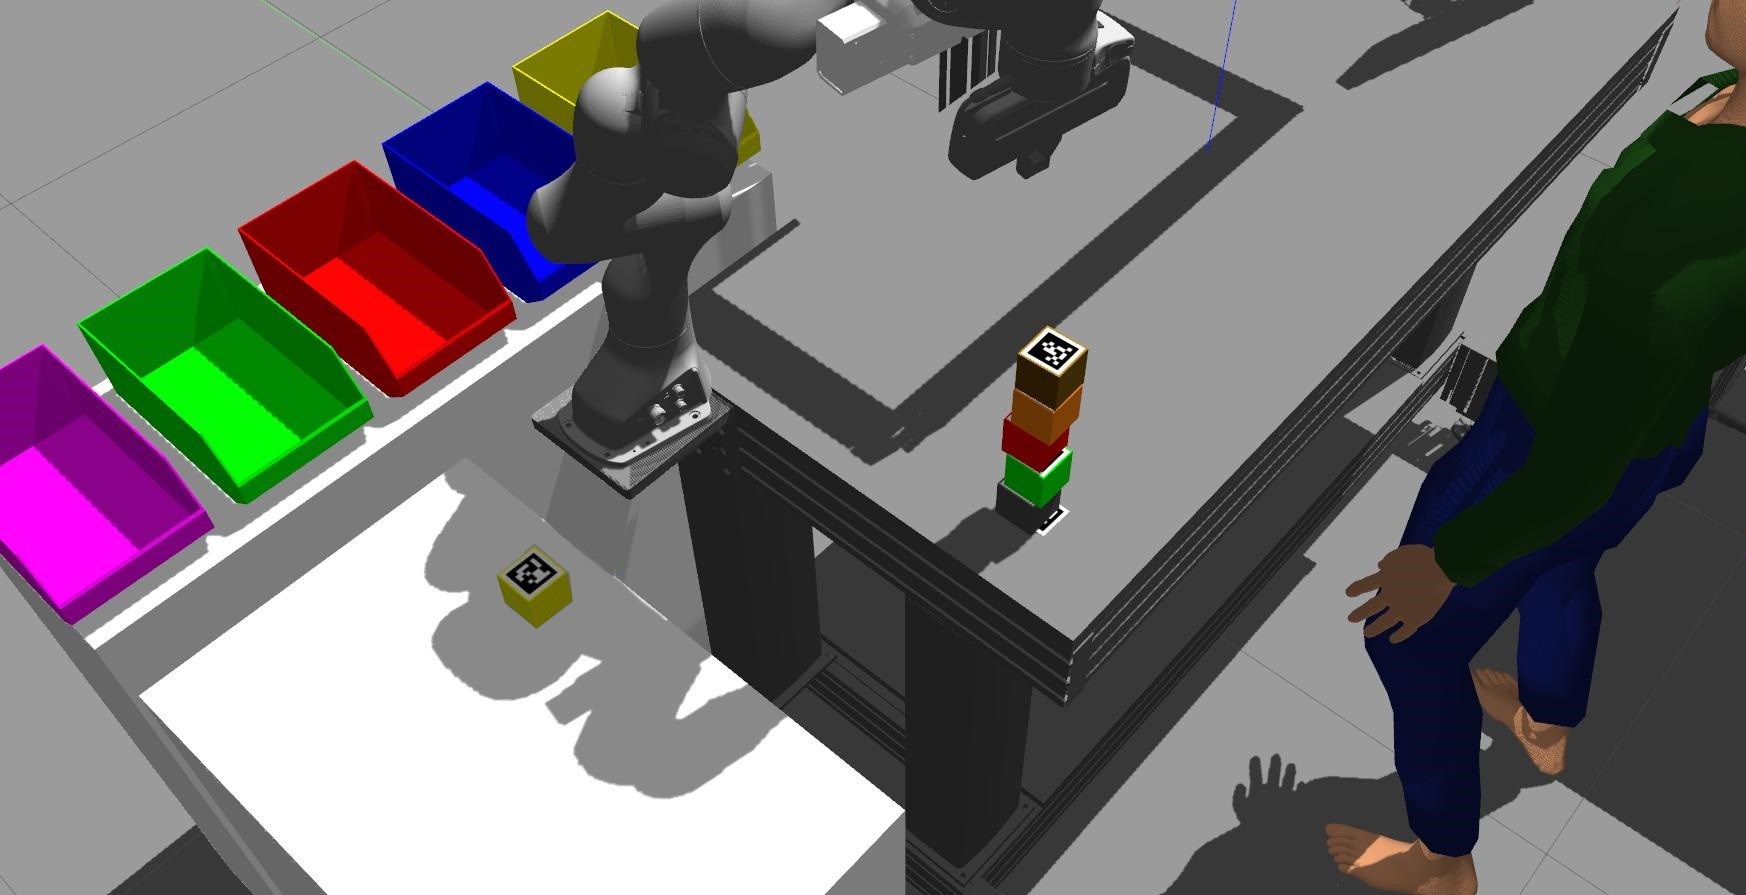
\includegraphics[width=0.6
\textwidth]{figures/Magistrale/ass_4}
\caption[Second Part of BlockB Assembly Simulation]{Assembly of BlockB on the workbench completed. 
\label{fig:ass_4}}
\end{figure} 


\section{Performance Considerations}\label{sec:perf_consid}

For this project, it is used a computer with Intel(R) Core(TM) i5-9300H CPU, NVIDIA GeForce GTX 1650 Max-Q graphics card and 8GB of RAM. 
The operating system, Ubuntu 18.04, is installed on an external SSD connected with the USB 3.1 standard. \\
The main performance issue comes from this setup. As described in the previous sections, the AtomSpace is an in-RAM knowledge representation database, which means it is completely contained in RAM. In addition, running the Ubuntu system on an external SSD also increases RAM occupancy. 
The combination of these factors constantly pushes RAM to the limit and the swap area does not work effectively, as data must pass through a USB connection, severely degrading performance. \\
Another aspect is the design of OpenCog: first of all, it is still in the development phase and it is only a few years since important considerations on the performance side are being made.